%%%%%%%
%%%%%%% Chapter 1
%%%%%%%
\chapter{Stochastic Simulation Methods}

Among the numerical techniques available to computational physics,
stochastic methods, also called Monte Carlo methods, play a 
central role. They are particularly appealing because of their 
immediacy, their power and the breadth of applications.

Monte Carlo methods rely upon the use of random 
numbers. Essentially there are two complimentary reasons to use
stochastic simulation methods:
the most obvious reason is the study of physical systems in 
which random events arise naturally; the second reason is that the 
sampling of random numbers offers an efficient numerical method 
to compute multidimensional integrals.

In order to elucidate the two important points just mentioned
we consider in the following two simple examples.

%%%%%%%%%%%%%%%%%%%%%%%%%%%%%%%%%%%%%%%%%%%%%%%%%%%%%%%%%%%%%%%%%
\section{The Radioactive Decay}
As an example of a natural stochastic process we consider radioactive decay.
Many  heavy nuclei are intrinsically unstable and decay to 
lighter, more stable elements
under the emission of $\alpha$--, $\beta$--, or 
$\gamma$--radiation. The radioactive decay is a statistical 
process. One can not forsee at what time the next nucleus will 
decay. According to the radioactive decay law one can predict the 
mean number of nuclei, which will decay in a given time interval.
Let us denote by $\lambda$ the decay constant, i.e., the fraction 
of given nuclei decaying per second, then the average number of 
decays occurring between time $t$ and time $t+dt$ is given by the 
relation
\begin{equation}\label{DECAY_LAW}
  dn = -\lambda n dt.
\end{equation}
The quantity $dn/dt$ is called the activity. Its dimension is the 
Becquerel (1Bq = 1s$^{-1}$). To give an example, the activity of 
1g of Radium $~^{226}_{88}$Ra is approximately equal to
$3.7 \cdot 10^{10}$ Bq (In an older notation the same activity was 
named 1 Curie). $\tau=1/\lambda$ is the mean life time, during 
which the number of radioactive nuclei drops to $1/e$.

If at time $t=0$ we have $n_0$ nuclei, it follows from Eq. 
(\ref{DECAY_LAW}) that at the later time $t>0$ we are left
with
\begin{equation}\label{DECAY_NUMBER}
n(t) = n_0 \exp(-\lambda t).
\end{equation}
The half--life $t_{1/2}$ is easily evaluated from the condition
\begin{equation}\label{HALF-LIFE_1}
  n(t_{1/2}) = \frac{n_0}{2}
\end{equation}
to be
\begin{equation}\label{HALF-LIFE_2}
  t_{1/2} = \frac{\ln2}{\lambda}.
\end{equation}
It is important to remark that for each nucleus
regardless of the decay mode $\lambda$
and $\tau$ are characteristic constants which do not depend upon, 
e.g.,
the temperature, the pressure, or chemical reactions.

Let us now turn our attention to the stochastic description of 
radioactive decay from which we will derive a stochastic 
algorithm. As we have already noticed a basic ingredient of all
Monte Carlo recipes is the use of random numbers. Thus, we have to 
know how to draw random numbers in our computer program. At the 
moment it is not important for us to know how random numbers can 
be generated. This will be the subject of one of the next 
chapters. We only have to know that almost all programming
languages have a random number generator in form of some function 
in their mathematical library. Shortly we will see how this can be
achieved in Java.


Let us assume that the system is made of $N_0$ 
unstable nuclei. The probability $p$ for a nucleus to decay in the 
finite time interval $\Delta t$ is obviously given by
\begin{equation}\label{DECAY_PROB}
  p = \lambda \Delta t \;\;\;  ({\rm for} \quad \lambda \Delta t \ll 1).
\end{equation}
Therefore it is easy to decide whether a nucleus decays with 
probability $p$ or not. To do so we have to draw a random number $R$
uniformly distributed in the interval $[0,1)$. This random number 
lies with probability $p$ in the interval $[0,p\Delta t]$. 
Therefore, if $R \leq p \Delta t$ a decay takes place, 
otherwise it does not. Hence in each time step $\Delta t$ we have to 
decide between two cases:
a) If a decay takes place we put $N \longrightarrow N-1$ and 
$t \longrightarrow t+\Delta t$; b) If no decay takes place we set 
simply $t \longrightarrow t + \Delta t$.

Thus, schematically the stochastic algorithm to simulate the 
radioactive decay reads

\begin{verbatim}
For t=0 to t with step dt
    For each remaining  nucleus
        Decide if the nucleus decays
        if (random number < p dt) then
              N ---> N-1
        end
    end loop over nuclei
end loop over time
\end{verbatim}

Before writing a program in Java to simulate the radioactive decay, let
us briefly discuss the generation of random numbers in Java.

\subsection{Random Numbers in Java}
In the introduction we have already met different possible ways to generate
random numbers in Java. The first method  \verb|random()| we encountered 
was contained in the \verb|Math| class of the \verb|java.lang| package.
The method \verb|random()| creates a single Random object the first time it
is invoked and returns pseudo-random numbers for that object for each
subsequent call. A better way to generate random numbers is provided by the
\verb|java.util| package, which contains several standard utilities
interfaces and classes. This second possibility is to be preferred since it
offers more possibilities to control the generation of random numbers. With
the help of 
\begin{verbatim}
public Random()
\end{verbatim}
we can create a new Random object. As we will learn in the next Chapter
the sequence of random numbers begins with the so--called seed.
The class Random automatically chooses a seed according to the current time.
If a specific seed is desired, this can be fixed
with the help of \verb|public Random(long seed)|.  
Furthermore, the method \verb|public synchronized void setSeed(long seed)|
which can be invoked at any time resets the sequence of random numbers to
start from the given seed.
Having instantiated the
Random object a pseudo-random number uniformly distributed between 0.0
(inclusive) and 1.0 (exclusive) is returned by invoking 
\begin{verbatim}
public double nextDouble()
\end{verbatim} 
Similarly, the method \verb|nextFloat| may be invoked to generate uniformly
distributed random numbers of the \verb|float| type.
In later Chapters we will also need uniformly distributed integer valued 
random numbers. Such pseudo-random numbers between \verb|Integer.MIN_VALU| 
and \verb|Integer.MAX_VALUE| can be generated in Java with the
help of
\begin{verbatim}
public long nextInt()
\end{verbatim} 
Alternatively it is possible to invoke also the method \verb|nextLong()|,
which generates discrete random numbers uniformly distributed between 
\verb|Long.MIN_VALUE| and \verb|Long.MAX_VALUE|.
Later on we will write our own class which will contain a method to generate
an integer valued  random number between $0$ and $N$ 
(the \verb|nextInteger()| method of the \verb|Distribution| class).
In Java 2 there is already a method \verb|nextInt()| to produce 
an integer valued random number between 0 and N. If you use Java 1.1
you can use our convenience method in the \verb|Distribution| class 
with the same name \verb|nextInt()|.

For later purposes, let us mention that the package \verb|java.util| also
contains a method
\begin{verbatim}
public synchronized double nextGaussian()
\end{verbatim}
which returns a pseudo-random Gaussian--distributed double value with mean 0.0
and standard deviation 1.0.

Now we are in the position to write a Java code for the simulation of
the radioactive decay.

\subsection{The Simulation Code}
The above algorithm written in Java is shown in the following listing.
\inputlisting{Listings_Java/RadioactiveDecay.java}

The program is straightforward. In line 6 to 11 the relevant variables 
are initialized. The main time loop starts is line 35 and the loop
over all the nucleiis starts in line 36. In line 38 we check if the
nuclei is already decayed or not. 
In order to check the results we evaluate the exact solution in 
line 41. Finally, we plot the result of the simulation to the 
screen comparing the exact with the simulated solution.

The class
\verb|RadioactiveDecay| has been written in such a way that it can be
run as an application as well as an applet. The trick is to extend the
\verb|Applet| class and to define, as it is necessary for
applications, a \verb|main| method. The actual algorithm is
implemented in lines 33 to 41.

We are now in the position to perform a simulation. To this end we
run the program with the following parameters
\begin{eqnarray*}
N_0 = 1000; \quad \lambda= 0.02 s^{-1}; \quad \Delta t = 1s; \quad 
 \verb|t_end| = 300s.
\end{eqnarray*}


Running the program it is evident that the screen output is not particularly
satisfactory to examine the results of the simulation. Thus, we have reached
the point where we feel the necessity to learn something about the graphical
possibilities of Java.


\subsection{The Most Easy Plot -- The AWT and Applet Packages}
\label{sec:AWTIntro}

Before trying to plot the data generated with the program
\verb|RadioactiveDecay| we want to discuss the most simple Java code which
allows to plot some 2 dimensional data. With the help of this example we will
learn the foundations of the graphical tools of Java. The code we want to
discuss is the \verb|PlotEasy| class which can be run as an applet or as
an application.

\inputlisting{Listings_Java/PlotEasy.java}

As we can see the code starts by importing packages. We already met the first
one, the \verb|java.applet.Applet| package in the applet version of the
HelloWorld program. The \verb|java.applet| package is a small package. It
simply contains the \verb|Applet| class, which is the superclass of all
applets, i.e., in order to create your own applet you have to create a subclass
of this class and override (overload) 
some or all of its methods (see chapter \ref{chap:IntroJava}). The
second package we have to import is the \verb|java.awt| package, where 
\verb|awt| stands for the Abstract Windowing Toolkit. This is one of 
the biggest packages in Java 1.1 and includes all the nice graphics
capabilities of Java.\footnote{The discussion is based on Java 1.1, but %
if you just prepend a capital \texttt{J} to all AWT class names, you can %
use the new Swing/Java 2 components. You also have to change the import %
command from \texttt{import java.awt.*;} to \texttt{import javax.swing.*;}. %
You should not use both together in one program.}

Java programs look different on different systems, because they use
the AWT, which is an abstract class, just defining the necessary
methods and fields to write programs using graphics functionallity.
To accomplish this, Java uses a so-called peer architecture, see figure
\ref{fig:peer}.
\begin{figure}[htbp]
  \begin{center}
    \leavevmode
    \setlength{\unitlength}{.8cm}
    \input{Figures/PeerArchitecture.pic}
    \caption{The peer architecture of the AWT in Java.}
    \label{fig:peer}
  \end{center}
\end{figure}

In order to understand the deep relation between applets and the AWT it is
instructive to look at figure \ref{fig:hierarchyapplet}, 
which shows the inheritance hierarchies of the Applet class.
\begin{figure}
  \begin{center}
    \leavevmode
    \setlength{\unitlength}{.8cm}
    \input{Figures/AppletHierarchy.pic}
    \label{fig:hierarchyapplet}
    \caption{This figure shows the inheritance hierarchy of the Applet class.}
  \end{center}
\end{figure}
Applets inherit the drawing and event handling methods from the AWT
\verb|Components| class. \verb|Component| is the superclass of all GUI
components in the \verb|java.awt| package. Many important methods
you have to use are defined in the Component class.

The \verb|java.awt.Container| class implements a component that contains other
components. \verb|Container| can not be instantiated directly. You always have
to use one of its subclasses, such as \verb|Panel|, \verb|Frame| or
\verb|Dialog|. Once a \verb|Container| is created you can set its Layout
Manager with \verb|setLayout()| or add components to it with \verb|add()|.
You can remove components with \verb|remove()|. 

The \verb|java.awt.Panel| class is a Container that is itself contained in a
Container. It does not create a separate window of its own. Applets are a
subclass of \verb|Panel| that is contained within a Web browser or an applet
viewer. Figure \ref{fig:awthierarchy} shows the hierarchy relations 
of some (not all!)
components and layouts classes of the \verb|java.awt| package.
\begin{figure}
  \begin{center}
    \setlength{\unitlength}{.65cm}
    \input{Figures/FrameHierarchy.pic}
  \end{center}
  \label{fig:awthierarchy}
  \caption{The hierarchy of the AWT package.}
\end{figure}

An important class of the AWT
package is the \verb|java.awt.Graphics| class, which encapsulates most of the
graphics functionality of the Java API. But the \verb|Graphics| class 
is an abstract class and does not have a constructor (For abstract classes,
please consult one of the books referenced in chapter 0). So there is no way
to instantiate a \verb|Graphics| object like \verb|new Graphics()| 
(This syntax is WRONG! Do not use it!).
To get a \verb|Graphics| object you can ask for one by calling
the \verb|getGraphics()| method of the \verb|Component| class (this is
only possible, if the actual \verb|Component| class does have a drawable 
graphic context, e.g. \verb|Canvas| or \verb|Container| objects). 
It makes obviously no sense to have a drawing area for a \verb|Button|
object for example. 
More common (and most of the time easier) is to overrride the
\verb|paint()| or \verb|update()| methods of a \verb|Component| object,
because both methods supply the \verb|Graphics| object a a parameter.

Now we have the necessary background to understand what is going on in the
\verb|PlotEasy.java| program. The class \verb|PlotEasy| extends the 
\verb|Applet| class and has a main method. In the \verb|main| method we
instantiate the \verb|Applet| \verb|PlotEasy|  and the \verb|Frame| \verb|f|.
The hierarchy of the \verb|Frame| class is (see Fig. \ref{fig:awthierarchy})
Object $\rightarrow$ Component $\rightarrow$ Container $\rightarrow$ Window
$\rightarrow$ Frame. The \verb|Frame| class represents an optionally resizable
application window with a title bar. 

With the help of the \verb|add(Component)| method in the 
\verb|Container| class,
we can ``add'' arbitrary components to our container. E.g. we can add
a button or a label to the frame we have created, for example:
\begin{sverbatim}
  Frame f = new Frame("Test Frame");
  Button but = new Button("Test"});
  ....
  f.add(but);  // here we add the Button to the Frame
  ....
  f.show(); // finally we show the Frame on the screen
\end{sverbatim}
The resulting window is shown in figure \ref{fig:ButtonDemo}.
\begin{figure}[htbp]
  \begin{center}
    \includegraphics[height=2cm]{Figures/ButtonDemo.eps}
    \caption{The output of the most easy window with a button using the AWT.}
    \label{fig:ButtonDemo}
  \end{center}
\end{figure}

A list of all AWT 
components defined in the Java 1.1 standard is shown in table 
\ref{tab:AWTComponents}.
\begin{table}[htbp]
  \begin{center}
    \begin{tabular}{c|p{0.6\textwidth}}
      Component & {\centering Usage} \\\hline\hline
      Button & A button with text on it. \\
      Canvas & A drawing area. \\
      Checkbox & A list of clickable choices (more than one can 
                 be choosen at a time). \\
      CheckboxGroup & A list of clickable choices 
                      (only one can be choosen at a time). \\
      Choice & A list of choices, like a pull-down menu. \\
      Label & A short text to be displayed in the GUI. \\
      Menu & Many components are available to realize menus.\\
      Scrollbar & Sometimes called a slider. \\
      TextComponent.TextArea & Multiple lines of text to be 
                               displayed or optionally editable.\\
      TextComponent.TextField & A line of text, optionally editable.\\\hline
      Container.Panel & A ``box'' to contain other components. \\
      Container.ScrollPane & A container to hold large areas, which cannot
              be displayed and have to be scrolled using the scroll panes. \\
      Container.Window.Frame & An optionally resizable window with 
                               title and decorations. \\
      Container.Window.Dialog & A dialog window to ask a question or display
                                a notification. \\
      Container.Window.FileDialog & For choosing/browsing files/directories. \\\hline\hline
      JRadioButton & A special Button (only one can be selected). \\
      
      JComboBox & Special purpose component to accomplish long lists.\\
      JList & A group of items displayed in a column.\\
      JSlider & For entering numeric values, which are bounded. \\
      JProgressBar & Visible component to show how much of a job has been completed.\\
      JColorChooser & Choose from a color box.\\
      JFileChooser & Get a file or path from the user. \\
      JTable & Display a table of data.\\
      JTree & Display hierarchical data.\\
      ToolTips & For every component you can have a balloon help/tool tip.\\\hline   
      Container.JToolBar & Group several components (eg. Buttons) with icons.\\
      Container.JSplitPane & Two panels in one. \\
      Container.JTabbedPane & Sharing the same place by many panels, similar to carlayout.\\
    \end{tabular}
    \caption{A list of most of the defined AWT components of 
      the Java 1.1 API and the
      Java2 API (Swing). In Java2/Swing all the AWT Components are also
      available with Swing by just adding a capital J to the beginning
      of the components (e.g. JButton instead of Button, JComponent instead
      of Component).}
    \label{tab:AWTComponents}
  \end{center}
\end{table}

The arrangement (in Java called layout) of the components and the containers
for each container can be defined by using a layout manager. By default it
always uses the \verb|FlowLayout| manager for an application, 
which just puts the components
beside each other in a line and if the window is too small it wraps them to
the next line. For an applet the default is the borderlayout manager.
More sophisticated layout managers are given in the 
table \ref{tab:AWTLayouts}. Unfortunately it is a pretty difficult
task to handle these layout managers, but still for not too complicated
arrangements it is enough to use these. If you want to have more
complex layouts and easier handling you should go and use the 
Swing/JFC packages (they are also available for Java 1.1 as mentioned
in the introductory chapter.). If you use an IDE like Simplicity for Java
or Netbeans, it is also easy to set up your own windows.
\begin{table}[htbp]
  \begin{center}
    \begin{tabular}{c|l}
      Layout Manager & how it works : \\\hline
      FlowLayout & The default layout, everything beside each other. \\
      GridLayout & Put all components/container in a table structure. \\
      BorderLayout & Use a center and 4 borders to put the components/containers.\\
      CardLayout & Put components/containers like cards on a stack.\\
      GridBagLayout & A very versatile but complicated layout manager. \\\hline
      BoxLayout & Components in a column, where the largest gives the width.\\
      ``Absolute Positions'' & New in Java 2, but it is better to use the others. \\
    \end{tabular}
    \caption{All possible layouts in the AWT package of Java 1.1.}
    \label{tab:AWTLayouts}
  \end{center}
\end{table}

Let us look back at the \verb|PlotEasy.java| program.
With the help of the method \verb|setSize(int width, int height)| we fix the
dimensions of the frame (in pixels). Another useful method is the 
\verb|pack()| method of the \verb|Frame| class, which sets the size
of the frame to the size necessary to display all contained components
of the frame. 
The \verb|show()| method displays the
frame. As we already know \verb|a.init()| calls the \verb|init()| 
method of the Applet class and therefore starts the applet. There is also
a method called \verb|setResizable(boolean)| for the Frame class, which
decides if the window can be resized by the user or not.

In principle the part of the code we just described is not necessary. We
included it only to allow the program to be run as an application and as 
an applet. Try to run the code without the lines 8 to 15 as an 
applet and it will still work, but it will no longer work as an
application, because the \verb|main| method is missing.

The actual plotting is performed by the \verb|paint()| method, which draws
on the screen (to be exact: in the panel of the Applet class). 
Applets typically override some of the methods of the
\verb|Component| class of the \verb|java.awt| package (you have
to override at least the \verb|init()| method, as we have already learned).
The simplest way for a Component to draw itself is
to put drawing code in the \verb|paint()| method. In lines 24 to 27 we see a
simple example of implementing the \verb|paint()| method. The \verb|Graphics|
class of the \verb|java.awt| package 
defines methods for drawing different kinds of shapes. The method which
we use here is the
\begin{sverbatim}
  drawLine(int x1, int y1, int x2, int y2)
\end{sverbatim} 
method, which simply draws a line with the current color 
in the \verb|Graphics| object \verb|g|. 
Other typical methods are shown in table \ref{tab:GraphicsMethods}.
\begin{table}[htbp]
  \begin{center}
    \begin{tabular}{c|p{3.2cm}}
      Method & Purpose \\\hline\hline
      \verb|drawLine(x1, y1, x2, y2)| & Draw a line or point.\\
      \verb|drawRect(x, y, width, height)|& Draw a rectangle \\
      \verb|fillRect(x, y, width, height)| & Draw a filled rectangle. \\ 
      \verb|clearRect(x, y, width, height)| & Clear a rectangle area. \\ 
      \verb|drawArc(x,y,width,height,Angle0,arc)| & Draw a part of a circle. \\
      \verb|fillArc(x,y,width,height,Angle0,arc)| & Draw and fill the arc. \\
      \verb|drawPolygon(int[] x, int[] y, nPoints)| & 
         Draw a polygon with the given points. \\
      \verb|fillPolygon(int[] x, int[] y, nPoint)| & 
         Same, but fills it with a color.\\    
      \verb|copyArea(x, y, width, height, dx, dy)| & Copy an area by dx/dy.\\
      \verb|drawString(String text, x,y)| & Draw text at the position.\\
      \verb|translate(x,y)| & Translate the origin. \\
    \end{tabular}
    \caption{List of some of the methods contained in the Graphics class.
      All method arguments are of type integer, unless otherwise stated.
      More methods are available in the much more powerful Java2D API
      coming with Java2.}
    \label{tab:GraphicsMethods}
  \end{center}
\end{table}
There is no drawPoint() method as you
might expect, but you can easily use the \verb|drawLine()| method 
with same starting and endpoint of course. Much more graphics
capabilities have been added by introducing the Java2D package
into Java2.



The  method \verb|getsize().height| and \verb|getSize().width|, which we use
in lines 19 and 25 return the height and the width of the Frame or
the panel of the applet.
Now that we understand the code let us run the program, either from the
command line or using the appletviewer or netscape.

If you try to resize the window, you realize that the plot is drawn
again and zoomed to the new window size. This is because we have not
overloaded the \verb|update()| method and the default behaviour of the
\verb|update()| method is to call the \verb|paint()| method again. In 
chapter 0 we have learned, that the \verb|update()| method is called
everytime the windows has to be redrawn, because of some events like
scolling in the browser window or, like here, resizing the window
(see figure \ref{fig:PaintMethod}.).
\begin{figure}[htbp]
  \begin{center}
    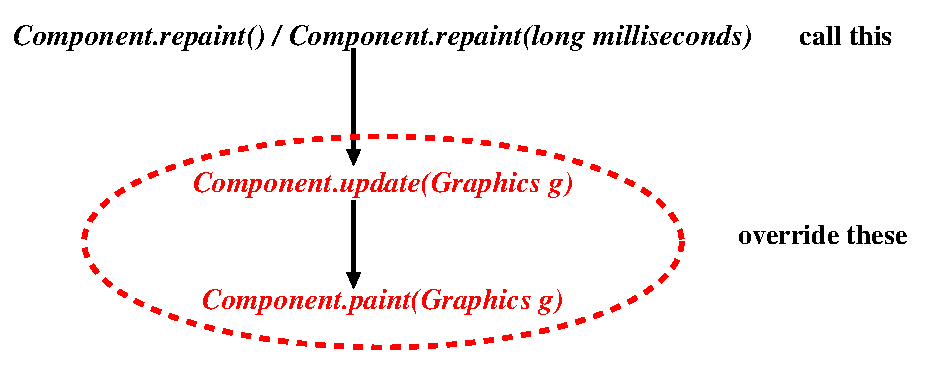
\includegraphics[width=\textwidth]{Figures/PaintMethod.eps}
    \caption{The default behaviour of the painting methods of components in the AWT package.}
    \label{fig:PaintMethod}
  \end{center}
\end{figure}

Having learned the basic graphical tools of the AWT with the help of
the most easy plot program, we can now apply what we have just learned
to the simulation of the radioactive decay.
\inputlisting{Listings_Java/RadioactiveDecay_easyplot.java}
Implementing the graphical facilities in the
\verb|RadioactiveDecay.java| code is easy. The output of 
the new program can be seen in figure \ref{fig:RDEasyPlot}.
\begin{figure}[htbp]
  \begin{center}
    \includegraphics[angle=-90,width=\textwidth]{Figures/RadioactiveDecayEasy.eps}
    \caption{The output of the easyplot version of the radioactive 
      decay program.}
    \label{fig:RDEasyPlot}
  \end{center}
\end{figure}

In the program code we immediately recognize
in the lines  56 to 81 the \verb|paint()| method. The results of the
simulation have to be scaled appropriately to fit in the Frame. The
curve is plotted with the method \verb|drawLine()|. Since we want to
plot also the exact analytical solution for the mean values in red we
set
\begin{verbatim}
  g.setcolor(Color.red)
\end{verbatim}
in line 74 before drawing the corresponding curve.

It is important to note that in the lines 21 to 24 
we have added the code
\begin{verbatim}
  frame.addWindowListener(...);
\end{verbatim}
which allows to handle the request to close the window. These ``events''
are in the \verb|java.awt.event| package and will be discussed later
in chapter \ref{sec:AWTAdvanced}. 

\subsection{Ptplot -- Extending Javas Graphics Capabilities}
The quality of the plot of the simulation results are rather poor
compared to high standards we are used to today. It is clear, that we
could now go on refining the plot with the help of the Java
AWT. Although this might be an interesting and instructive task, it is
not our primary interest in this book. Fortunately, there are advanced
2D graphics components which can be used in applets and
applications. One of these packages is Ptplot (you pronounce it
pee--tee--plot). The Ptplot package is released under the liberal UC
Berkley copyright. It has been developed by Edward A. Lee, C. Hylands,
and W. Wu. You are free to download it at
\href{http://ptolemy.eecs.berkeley.edu/java/ptolemy.plot2.0/ptolemy/plot}%
         {http://ptolemy.eecs.berkeley.edu/java/ptolemy.plot2.0/ptolemy/plot}
where you also find
the documentation and many demos of Ptplot. 

The components of Ptplot have the following properties:
\begin{itemize}
\item plots are embeddable in applets and applications
\item you may use binary or ASCII data
\item the plots are auto--ranging
\item you may label automatically or manually the axes
\item logarithmic axes
\item live, animated plots
\item infinite zooming
\item  various plot styles (connected lines, scatter plots, bars, ..)
\item various point styles (none, dots, points, ....)
\item multiple data sets and legends
\item color or black and white plots
\item error bars.
\end{itemize}
Before writing the first program using Ptplot take a look at the
class hierarchy of Ptplot in figure \ref{fig:PtplotHierarchy}.
\begin{figure}[htbp]
  \begin{center}
    \leavevmode
    \setlength{\unitlength}{.8cm}
    \input{Figures/PtplotHierarchy1.pic}\\[.3cm]
    \input{Figures/PtplotHierarchy2.pic}
    \caption{The class hierarchy of the Ptplot package.}
    \label{fig:PtplotHierarchy}
  \end{center}
\end{figure}

Let us now look at a very simple program in order to demonstrate
what you need to invoke the Ptplot methods.
\inputlisting{Listings_Java/Ptplot_Demo1.java}

We see that we have to import additionally the  Ptplot package. The
class \verb|ptplot_Demo| extends the class \verb|PlotApplet|. Again we
want to run the code as applet as well as an application so the class
does have a main method. In lines 14 to 17 we instantiate the new Frame
and activate the WindowListener as we did it in the
\verb|RadioactiveDecay_ploteasy.java| code. The actual plot routines
are in lines 28 to 33. In the \verb|init()| method we invoke the method
\verb|super.newPlot()| to create a new plot, \verb|super.init()| to
initialize it and \verb|plot().setTitle| to give the plot a title.

A second possibility of using Ptplot, which we prefer to use, is to extend
the \verb|Applet| class instead of the \verb|PlotApplet| class and 
change the lines 28 to 33 to:
\lstinputlisting[first=28,last=33]{Listings_Java/Ptplot_Demo2.java}
The difference is that the \verb|PlotApplet| class realizes a kind
of interface for an applet to start plot commands confirming to the
pxgraph commands and executes them from parameters given in the applet.
Pxgraph is a program for the X windows system to plot data using
batch files like gnuplot. The full pxgraph functionality is
included in the ptplot package and can be used. For further documentation
concerning this point, please refer to the ptplot documentation.

Next we want to draw the results of the simulation of the radioactive
decay process with the help of Ptplot and learn at the same time how
to exploit the features of Ptplot. The corresponding code can be seen
below.
\inputlisting{Listings_Java/RadioactiveDecay_ptplot.java}
The output of the code can be seen in Fig. (\ref{fig:ptplotOutput}). 
\begin{figure}[htbp]
  \begin{center}
    \leavevmode
    \includegraphics[angle=-90,width=\textwidth]{Figures/RadioactiveDecay_ptplot.eps}
    \caption{The output of the RadioactiveDecay\_ptplot.java program.}
    \label{fig:ptplotOutput}
  \end{center}
\end{figure}

The actual plotting code starts in line 55 and ends in line 79. 
There we use several methods of the \verb|ptplot.Plot|
class and of the superclass \verb|PlotBox| of the \verb|Plot| class.
All methods are called \verb|setMethod| where \verb|Method| is
self-explaining. Several other methods are implemented in the
\verb|Ptplot.PlotBox| class and its child, the \verb|Ptplot.Plot| class. 
They are summarized in table \ref{tab:PtplotMethods}. 
\begin{table}[htbp]
  \begin{center}
    \small
    \leavevmode
    \begin{tabular}{p{5cm}|p{8cm}}
      Method & Purpose \\\hline\hline
      \verb|addLegend(int, String)| & draw a legend for one plot number\\
      \verb|addXTick()| & \\
      \verb|addYTick()| & \\
      \verb|setBackground(Color)| & set the background color of plot\\
      \verb|setForeground(Color)| & set the foreground color of plot\\
      \verb|setGrid(boolean)| & draw a grid \\
      \verb|setLabelFont(String)| & font for axis labels and legend labels  \\
      \verb|setTitle(String)| & title of graph \\
      \verb|setTitleFont(String)| & set title font \\
      \verb|setXLabel(String)| & label of x axis \\
      \verb|setYLabel(String)| & label of y axis \\
      \verb|setXLog(boolean)| & x axis logarithmic scaling \\
      \verb|setYLog(boolean)| & y axis logarithmic scaling \\
      \verb|setXRange(double, double)| & x range of the plot \\
      \verb|setYRange(double, double)| & y range of the plot \\\hline
      \verb|addPoint(int, double, double, boolean)| & add a point to the plot,
      the boolean var. decides, if the point gets connected with the last one.
      The integer var. is the plot number.\\
      \verb|addPointWithErrorBars(int,| 
                     \verb|double, double, double, double, boolean)| & %
      add a point to the plot with errorbars. Th additional vars. specify the
      lower and higer y coordinate of the error bar.\\
      \verb|setBars(boolean)| & bar plotting on or off \\
      \verb|setBars(double, double)| & define width and offset for bar 
      plotting and enable bar plotting. \\
      \verb|setImpulses(boolean)| & plot impulses \\
      \verb|setMarksStyle(String)| & none, points or various \\
    \end{tabular}
    \caption{Overview of all the Ptplot methods in the Plot and PlotBox classes.}
    \label{tab:PtplotMethods}
  \end{center}
\end{table}

Although this is the most common way of using ptplot in this book, there
is another feature coming with ptplot. It can read data files and plot
the data. For this you have to write a script, which contains the
commands for the plot to be created. This scripting language
is borrowed from the \emph{pxgraph} program. It is like using ``gnuplot''
 with
its scripting facilities. For details you can look at the 
documentation coming with the ptplot package. For us it will be
easier to read the files into Java and then use ptplot to plot it on 
screen.

%%%%%%%%%%%%%%%%%%%%%%%%
\subsection{3D plots in Java -- Java3D}
Sometimes you are forced to use 3D plots to visualize your data
and therefore it is natural to ask for a package to accomplish
three dimensional plots. Unfortunately to our knowledge there is
(yet) no freely available package in Java for 3D plots. Ptplot
can only handle 2D plots and JSci can handle only some very
basic 3D plots (see chapter \ref{sec:JSci}).

There is also a program called 
\verb|SciVis|\footnote{\href{http://kopernik.npac.syr.edu:8888/scivis/}%
  {http://kopernik.npac.syr.edu:8888/scivis/}},
which is completely written in Java and allows for 2D and 3D plots
in many different ways. But up to now, there are only C and
Fortran interfaces to supply data to it. You can also read from
files, but first you have to understand the data format, which is
described in the users guide.
The authors told us they are developing a Java interface to
supply data directly to \verb|SciVis|. 

At the moment, the best solution is to write the data to a file
and use an external program available to you. The most common
denominator would possibly be ``gnuplot'', which is available for many
different platforms and can create a lot of different 3D plots.

Since Java 2, there is a new (external) API -- not included in the JDK 1.2
disribution, you have to get it seperatly -- called \emph{Java3D}. 
This is a full implementation of three dimensional routines to
produce all kinds of 3D scenes and objects and even move these scenes.
With this API it seems to be possible to write a fairly easy
3D plotting program in the near future. So this lack of features
in Java for the scientist should be gone soon. 

%%%%%%%%%%%%%%%%%%%%%%%%%%%%%
\subsection{Using (system dependent) external programs like gnuplot}
There is a last way of obtaining 3D plots ``in Java'': You can use
an external program like Gnuplot or any other command line tool and
call it from a Java program. This of course is not system independent
and is not recommended unless you are desperatly needing it.

In Java there is a class called \verb|Runtime| in the \verb|java.lang|
package, which consists of all kind of methods to change and
use the environement you are running your Java program in. This can be used
to start a subprocess of the running Java program. So starting an
external process from a Java program can be done in two steps:
\begin{itemize}
\item Get a \verb|Runtime| object of the running Java program.
\item Start a new process as a subprocess of the given \verb|Runtime| object.
  You have to use the \verb|exec(String)| instance method of the  \verb|Process|
  class for this. 
\end{itemize}
You can also read the standard output of the subprocess and use it in your 
Java program. To demonstarte how it actually works, we give two examples:
\begin{enumerate}
\item A Java program starts a Gnuplot program, which plots a sine curve.
  \inputlisting{Listings_Java/Gnuplot.java}
\item A Java program executes a ``ls -al'' command on a UNIX machine,
  which just gives the directory listing. For a Windows system you just
  use the ``dir'' command instead.
  \inputlisting{Listings_Java/DirectoryListing.java}
  This time we also wait for the execution of the process to finish and 
  then read the standard output and display it on the screen.
\end{enumerate}

%%%%%%%%%%%%%%%%%%%%%%%%%%%%
\subsection{Printing in Java and with Ptplot}
Now that we have learned how to make plots in Java, it is of great
importance to get a printed version of our graphics. For
this purpose Java has commands for initiating a print job and preparing
the output for the printer. Java always produces potscript output.
Because the procedure has changed
from Java 1.1 to Java 2, we only present the Java 1.1 version not
to confuse you. In Java 1.0 there have been no methods for 
printing in  Java, you would have to use screen capture programs
for example.

Because printing is of course system dependent, it is not as easy
as issuing a print command, but it is still managable. 
In Java printing is done basically in four steps:
\begin{enumerate}
\item Get a \verb|Toolkit| for the component you want to print. 
  Use method \verb|getToolkit()| in the \verb|java.awt.Component| class.
\item Get a \verb|PrintJob|. Use the 
  \verb|getPrintJob(Frame f, String printjobname, Properties printprops)|
  method in the \verb|java.awt.Toolkit| class.
\item Start ``printing'':
  \begin{enumerate}
  \item Get the graphics context for the component in question. Use the
    \verb|getGraphics()| method of the \verb|java.awt.PrintJob| class.
  \item Print the desired part of the component. If you want to print 
    everything contained by the component use the \verb|printAll()|
    method, otherwise use just the \verb|print()| method of the
    \verb|Component| class.
  \item Send the data to the printer or file by using the \verb|dispose()|
    method of the \verb|java.awt.Graphics| class.
  \end{enumerate}
\item Finish printing and close dialog box. Use \verb|end()| method of
  the \verb|java.awt.PrintJob| class.
\end{enumerate}
The program \verb|RadioactiveDecay_printing.java| demonstartes the use of
the printing capabilities of Java. 
\lstinputlisting[first=32,last=47]{Listings_Java/RadioactiveDecay_printing.java} 

Of course there are some drawbacks to talk about. First of all with
this code you always get the output in a size referring to your actual
picture on the screen, it does not use the full paper size. If you want
to use the whole page size available you have to scale the component
to be plotted to the full size and scale back after printing. This is
what we do in the convenience class we have written for easy printing
in the simulation package. 

So if you want to print a component scaled to the full size, you use
the \verb|PrintComponent.Dialog()| method in the simulation package.
It scales your component to the full size -- no matter if it should be
on a portrait or landscape page -- and sends the scaled picture to the
printer or a postscript file. After printing it scales back to the
size it had before. The whole code above could therefore be
substituted by the line
\begin{verbatim}
  import simulation.*;
  ....
  PrintComponent.Dialog(frame, plot, "Radioactive Decay");
\end{verbatim}
Because most of the time you need postscript (or EPS) files of the
created plots or graphics, this is the most common use of the
printing features for a scientist.

A second method of the \verb|simulation| class called \verb|DialogNoScaling()|
can be used to produce unscaled output of the component or container.
I thas the same syntax as the \verb|Dialog()| method before.

There is one caveat to mention: if you are going to insert the
produced postscript files into TeX/LaTeX, you will have to do
some editing on the postscript files. First of all you have to
add a bounding box line at the beginning of the postscript
file. You can do this by hand, put a line (for a portrait figure)
\begin{verbatim}
 %%BoundingBox:  0 0 595 840
\end{verbatim}
at the beginning of the postscript file (You can adapt the numbers
to the figure at hand and check the area by viewing it in 
ghostscript/ghostview.) or you can use a program to automatically
calculate and insert a bounding box command (like e.g. epstool,
gsview on Windows, etc.). The second change is to remove all the 
lines between \verb|%%BeginSetup| and \verb|%%EndSetup| except
a possible rotate line like \verb|90 rotate 0 -595 translate|.
This is necessary, because some strange effects appear in the
resulting \verb|.dvi| or \verb|.ps| file after "texing".

Another drawback might be the resolution of the postscript file.
This happens especially when printing GUI components and is not
present when plotting ptplot plots fortunately. Java kind of rasters
the screen display and because the screen resolution is much worse 
than the printer resolution this gives unpleasant results. It also
gives strange results if you scale a large GUI to a small A4 or Letter
format for printing, which could look very ugly or even miss some
of the displayed objects. But as already mentioned, most of the time
we only need plots in postscript files and this works great with
the code above.

In Java 2 there has been some small changes to the printing
interface. A new class has been introduced in Java2: \verb|java.awt.print|.
This class provides much more sophisticated methods and it is even
able of handling color models, which is very important for
color handling and printing. This is a big step ahead, but for the
details we refer to the API documentation, because it is also a
bit more difficult to understand.

Ptplot 2.1 printing facilities ????? (EPS)

\paragraph{Printing from an Applet}
Usually applets are not allowed to initiate printjobs, unless
a \verb|SecurityManager|, another important Java class, explicitly
allows for it. Most of the time the browser or appletviewer has
to initiate the printjob, allowed by the security manager. You can of
course always use the printing facilities of the browser and plot
the whole panel visible in the browser.


What you can do is, write a main method in the applet and start
it as an application. Do the plots  and print them from the
application. 

If you use a security manager and are allowed to print, you need a
frame for your applet, because the  \verb|getPrintJob()| command
only takes a frame and not an applet as first argument. So just
put a frame into the applet and then put the applet inside the frame.


%%%%%%%%%%%%%%%%%%%%%%%
\subsection{The Results of the Simulation}

The results of the simulation are plotted in Fig. (\ref{FIG_DECAYA}) and 
(\ref{FIG_DECAYB}).
\begin{figure}
\label{FIG_DECAYA}
\begin{center}
\includegraphics[angle=-90,width=8cm]{Figures/RadioactiveDecay_1.eps}\\
\includegraphics[angle=-90,width=8cm]{Figures/RadioactiveDecay_2.eps}
\end{center}
\caption{Two realizations of the stochastic process of the radioactive decay.
The first one with linear y axis scaling and the second one uses a logarithmic
y axis scaling. The blue lines are the exact solution and the red ones
are the simulations.
The parameters of the simulation were choosen to be $N_0 = 100; 
\quad p = \lambda \Delta t = 0.01 s^{-1}; \quad \Delta t = 1\text{s};
\quad t_{\text{end}} = 300\text{s}$}
\end{figure}
\begin{figure}
\label{FIG_DECAYB}
\begin{center}
\includegraphics[angle=-90,width=11cm,clip]{Figures/RadioactiveDecay_3.eps}\\
\end{center}
\caption{The same as figure \ref{FIG_DECAYA}, but with different parameters:
$N_0 = 1000; \quad p = \lambda \Delta t = 0.03 s^{-1}; 
\quad \Delta t = 1\text{s};  \quad t_{\text{end}} = 100\text{s}$}
\end{figure}
 It is 
immediately recognized that the simulation results fluctuate around 
the expected curve. This is of course not astonishing since the 
exact result holds for mean values. In order to achieve a better
agreement with the decay law it is necessary to run the simulation
several times and to take the average over the different 
realizations of the decay process. This can easily be achieved by 
a simple modification of the program \verb|RadioactiveDecay_ptplot.java|.
 We introduce an additional input variable, the number of realizations
\verb|nreal| and accordingly implement a loop over the different 
realizations. This can be best seen in the listing of the 
new program \verb|RadioactiveDecay_ptplot2.java|.
\lstinputlisting[first=61,last=63]%
          {Listings_Java/RadioactiveDecay_ptplot2.java}

At the end of the realizations loop
we have to perform the average. This is seen in lines 61 to 63.
(STRESS MORE THE IDEA OF REALIZATIONS!!!!; allgemeine Strategie erlaeutern.)

Note that in order to speed up the program we have modified slightly 
the algorithm  so that we can save a loop. ?????
The probability to observe one decay in time $\Delta t$ is
\begin{equation}
p = \beta \Delta t
\end{equation}
where $\beta = \lambda N$ and $\Delta t$ must be small enough so 
that $\beta \delta t \ll 1$. 
From the elementary rules of combinatorics we know that
the probability to observe $n$ decays in time $t=m\Delta t$ is therefore
given by
\begin{equation}
P = p^n(1-p)^{m-n} {m \choose n}.
\end{equation}
Inserting the definition of $p$ the above expression can be cast 
in the form
\begin{equation}
P = \left( \frac{\beta t}{m}\right)^n 
     \left( \frac{1 - \beta t}{m} \right)^{m-n}
      \frac{m!}{(m-n)! n!}.
\end{equation}
Performing the limit $\Delta t \longrightarrow 0$ (i.e. $m 
\longrightarrow \infty$) and considering that
\begin{equation}
\left(1-  \frac{\beta t}{m} \right)^{m} \longrightarrow 
            \exp(-\beta t),
\end{equation}
\begin{equation}
\left( 1- \frac{ \beta t}{m} \right)^{-n} \longrightarrow 
            1,
\end{equation}
and
\begin{equation}
\frac{m!}{(m-n)! n!} \longrightarrow m^n
\end{equation}
we obtain the result
\begin{equation}
P = \frac{\mu^n \exp(-\mu)}{n!},
\end{equation}
where $\mu = \beta t$. The above distribution is the well know
Poisson distribution.

\subsubsection{Plot Methods in the Simulation Package}
Because sometimes it is easier to use ready made routines, we
have added some plotting convenience classes and methods to
get the plots faster. If you take the shortcut presented here
or you want to use the low level ptplot interface does not 
matter, it is totally up to you.

?????
\paragraph{plot2D()}
\paragraph{errorBars()}
\paragraph{histogram()}
\paragraph{barPlots()}

It is now easy to verify that the number of decays in a given 
interval is distributed according to the Poisson distribution.
To this end we have counted the number of decays in a given 
interval. This is accomplished in the lines xy. At the end of the
program we plot in a histogram the distribution of the number of 
decays and overlay the expected Poisson
distribution.  

\subsubsection{Listing of the full Program}
\lstinputlisting{Listings_Java/RadioactiveDecay_ptplot2.java}


Run the program for the following two sets of parameters:
\begin{eqnarray*}
N_0= 100, p = 0.001 s^{-1}, \Delta t = 1s, t = 100s \\
N_0= 100, p = 0.0001 s^{-1}, \Delta t = 1s, t = 100s
\end{eqnarray*}
with nreal = 100 and nreal = 1000.

The result of  two simulations can be seen in figs. x and y.
\begin{figure}
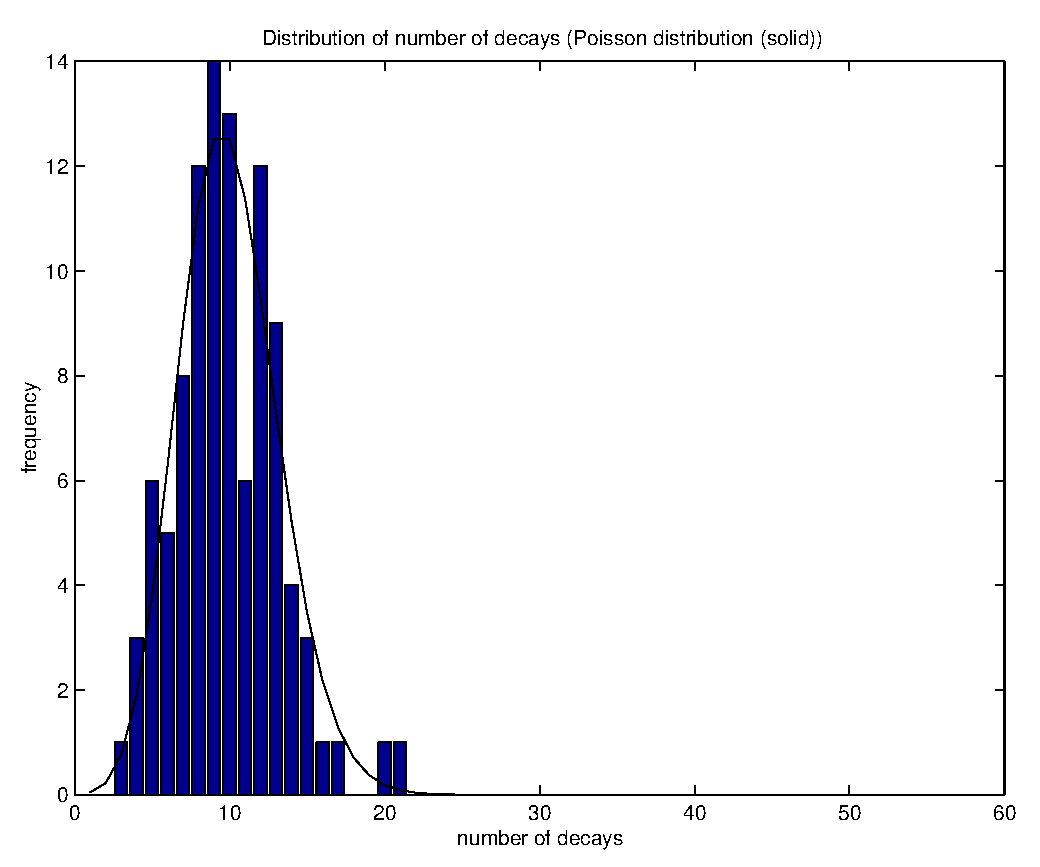
\includegraphics[width=\textwidth]{Figures/f_decay1.eps}
\caption{The distribution of the number of decays computed with 
the program decayr. 100 realizations. The simulation was run for
N0=100 and lambda=0.001.}
\end{figure}

\begin{figure}
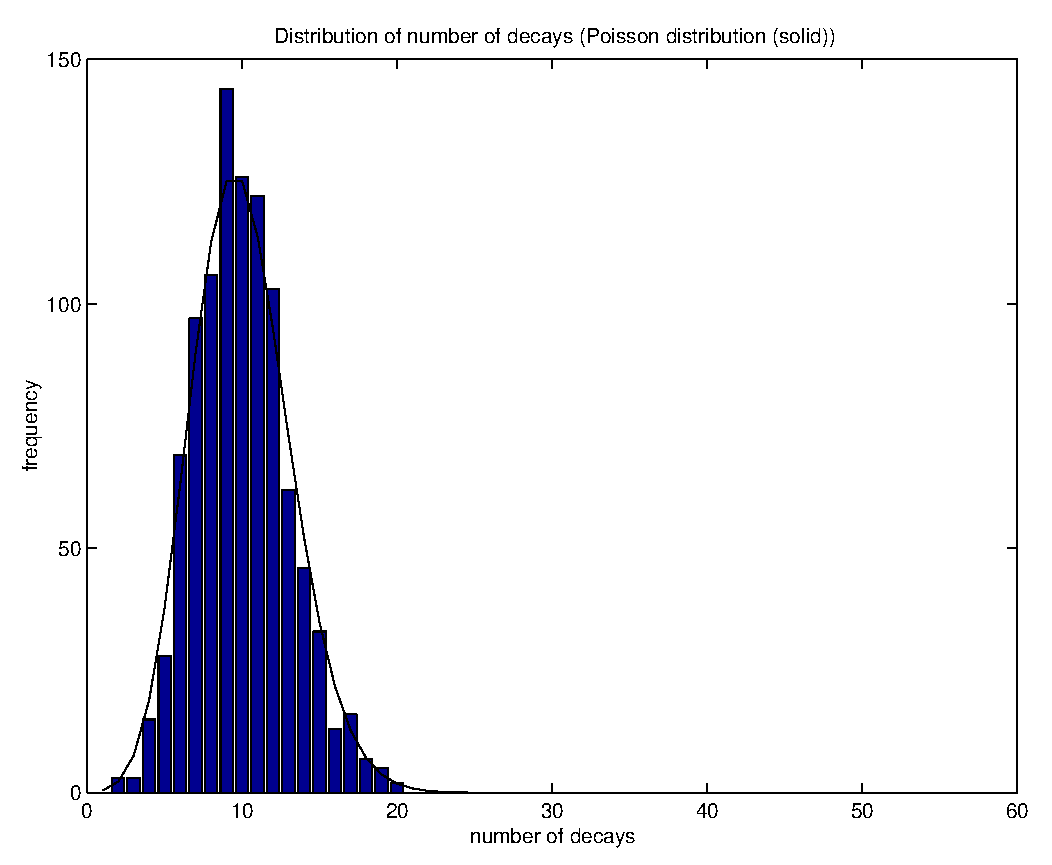
\includegraphics[width=\textwidth]{Figures/f_decay2.eps}
\caption{The distribution of the number of decays computed with 
the program decayr. 1000 realizations. The simulation was run
for N0=100 and lambda = 0.001.}
\end{figure}

%%%%%%%%%%%%%%%%%%%%%%%%%%%%%%%%%%%%%%%%%%%%%%%%%%%%%%%%%%%%%%%%%%%%%%
\section{Simple Monte Carlo Evaluation of Integrals}
It is the purpose of this subsection to introduce Monte Carlo Methods
in the context of the numerical evaluation of definite integrals.
We will see in later chapters that Monte Carlo integration is the
method of choice when treating multidimensional
integrals numerically. As a typical rule of thumb
``classical'' deterministic methods are outperformed
by Monte Carlo methods  for systems with a large number of 
degrees of freedom.
For simplicity and to stress the basic ideas 
it is convenient at the moment to consider one--dimensional definite
integrals of the form
\begin{equation}
\label{INTEGRAL}
I = \int_a^b dx f(x).
\end{equation}
Obviously such integrals can be evaluated analytically for many
integrands
$f(x)$.  However, there are as well many cases for which a numerical
evaluation is necessary.

Before introducing the Monte Carlo approach to numerical integration
let us remind the basic ``classical'' deterministic approach to
numerical integration. The standard approach is based upon the
geometrical interpretation of the integral (\ref{INTEGRAL}) as the
area under the curve of the function $f(x)$ between the points $a$ and
$b$. In the simplest algorithm this area (see figure) is approximated
as a sum over rectangles. To this end the $x$--axis is divided into
$n$ equally spaced intervals of width $\Delta x$,
\begin{equation}
\Delta x = \frac{b-a}{n}
\end{equation}
whose ends are given by
\begin{equation}
x_i = x_0 + i\Delta x
\end{equation}
for $i=1, \ldots ,n$. Of course, $x_0 = a$ and $x_n =b$. Thus in the
so--called rectangular approximation the integral is evaluated as
\begin{equation}
\label{I_CLASSICAL}
I_n = \Delta x \sum_{i=0}^{n-1} f(x_i).
\end{equation}
Of course, other more accurate approximations are possible.

How can we now evaluate the above integral by drawing random numbers?
The standard way is based on a very simple idea. 
From the introductory course in analysis we know that the Mean 
Value Theorem states that the exact value of the integral $I$ is 
given by
\begin{equation}
I= (b-a) f(\zeta)
\end{equation}
for some value of $\zeta$ in the interval $a \le \zeta \le b$. $f(\zeta)$
represents the average value of the function $f(x)$ 
in the interval $[a,b]$. Thus we could also write
\begin{equation}
I = (b-a) \langle f \rangle,
\end{equation}
where $\langle  \rangle$ denotes the mean value.
Let us draw $n$
random numbers which are uniformly distributed in the interval $[a,b]$
and let us sample the corresponding value of $f(x_i)=f_i$. The Monte Carlo
estimate $I_n$ of the integral $I$ is then the sample mean, which is
given by
\begin{equation}
\label{MCI_STANDARD}
I_n = \frac{(b-a)}{n} \sum_{i=1}^{n} f(x_i),
\end{equation}
where $n$ is the number of trials. Amazingly the form of the above
estimate is very similar to the classical formula (\ref{I_CLASSICAL}).
The fundamental difference is that now the $n$ points at which the
function $f$ is evaluated are no longer equally spaced but randomly 
distributed.

There is also the possibility to compute the integral $I$
stochastically
with the help of the ``Hit or Miss'' algorithm. The idea behind
this algorithm is again very simple. To be explicit we imagine a rectangle
of height $h$ and width $(b-a)$ such that the function $f(x)$ lies
within the rectangle (see figure; Gould, p.329). To evaluate the
integral we draw randomly pairs of uniformly distributed random
numbers $(x_i,y_i)$ such that $a \le x_i \le b$ and $0 \le y_i \le h$.
In other words the probability to draw a point within the rectangle is
given by the inverse of the area $A$ of the rectangle,
i.e. $1/(b-a)h$. It is now evident how the area under the
function $f$ may be estimated. The fraction of points $(x_i,y_i)$
which satisfy the condition $y_i \le f(x_i)$ is an estimate of the
ratio of the integral $I$ to the area $A$ of the rectangle. Hence,
drawing $n$ random pairs the estimate $I_n$ of $I$ by this ``scoring''
method is given by
\begin{equation}
I_n = A \frac{n_s}{n},
\end{equation}
where $n_s$ is the number of ``hits'', i.e., of points lying below the
curve $f(x)$.

Before writing two simple programs to elucidate the above algorithms
it is important to have in mind that both estimates are affected by
statistical errors. Let us consider for simplicity 
the standard method. Since the $f(x_i)$ are random we know 
from the elementary theory of data analysis
that an appropriate measure of the error is given by the variance
which is defined by
\begin{equation}
{\rm Var}(f) = \langle f^2 \rangle - \langle f \rangle^2.
= \langle (f -\langle f \rangle)^2 \rangle
\end{equation}
Since we draw a finite number of random numbers we can
estimate the mean value by using
\begin{equation}
\hat{f}  = \frac{1}{n} \sum_{i=1}^n f(x_i) 
\end{equation}
and correspondingly the estimate of the variance by using
\begin{equation}
{\rm Var}(f(x_1),\ldots, f(x_n)) = \frac{1}{n-1} \sum_{i=1}^n 
   (f(x_i)- \hat{f})^2 = \sigma_f^2.
\end{equation}
The quantity $\sigma_f = \sqrt{{\rm Var}(f_1, \ldots, f_n)}$ 
is also called the standard deviation. In the previous expression
we have used the short--hand
notation $f(x_i) = f_i$. However,
we are not interested in the error of $f$ but in the error of the
estimate $I_n$, which is a sum over random numbers. 

Repeating the 
simulation and hence drawing other random numbers we will get another
estimate of $I_n$. Therefore, repeating the simulation $m$ times 
we can estimate the mean of $I_n$ as
\begin{equation}
\hat{I_n} = \frac{1}{m} \sum_j^m I_n(j)
\end{equation}
and the corresponding variance as
\begin{equation}
{\rm Var}(I_n(1), \ldots, I_n(m)) = 
\frac{1}{m-1} \sum_j^m (I_n(j) - \hat{I_n})^2 = \sigma_I^2
\end{equation}
We will denote the above variance also by $\sigma_I^2$.
Of course, proceeding this way is not very practical since we
have to perform the simulation $m$ times. A much more economical
estimation of the error of the mean of $I_n$ could be achieved by 
establishing a simple relation between $\sigma_I$ and the standard 
deviation of the individual trials $\sigma_f$. To this end we 
introduce the discrepancy $\delta f_i$ between the
individual trial $f_i$ and its mean $\langle f \rangle$. The 
discrepancy $\delta I_n$ between $I_n$ and its mean value can be
obtained to first order in the $\delta f_i$ by a simple Taylor 
expansion (error propagation rules)
\begin{equation}
\delta I_n = \sum_{i=1}^n \frac{\partial I_n}{\partial f_i} \delta 
f_i.
\end{equation}
Hence, it follows from the above equation by taking the average over
$\delta I_n^2$ that
\begin{equation}
\langle \delta I_n^2 \rangle = \sum_{i,j=1}^{n}
    \frac{\partial^2 I_n}{\partial f_i \partial f_j} 
     \langle \delta f_i \delta f_j \rangle.
\end{equation}
It is plausible to assume, that 
$\langle \delta f_i \rangle = 0$
for all $i$ and that the $\delta f_i$ are not correlated
for $i \neq j$, i.e.,
$\langle \delta f_i \delta f_j \rangle = \langle f_i \rangle \langle f_j \rangle$
and that for $i=j$ we have $\langle \delta f_i^2 \rangle = \sigma_f$ 
for all $i$ it follows from the above equation that
\begin{equation}
\sigma_I^2 = \sum_{i=1}^n \left(
      \frac{\partial I_n}{\partial f_i} \right)^2 \sigma_f^2
      = \frac{1}{n^2} n \sigma_f^2 = \frac{\sigma_f^2}{n}
\end{equation}
and finally we have the useful relation
\begin{equation}
\sigma_I = \frac{\sigma_f}{\sqrt{n}}.
\end{equation}
The mean error of the mean scale with 1 over the square root of 
the number of individual trials. The precision of the estimate 
thus increases only slowly with the number of trials (remark: central
limit theorem: see Chapter 2).

Now we are in the position to write two programs to implement the above
stochastic algorithms. In order to be specific we compute the integral
\begin{equation}
I = \int_0^1 dx \sqrt{1-x^2} = \frac{\pi}{4}.
\end{equation}
In other words we want to estimate the number $\pi$ by Monte Carlo
methods.

We begin by the standard method. The listing of an according 
program can be seen below.

\subsubsection{Listing of the program mcpi.}
\inputlisting{./Listings/mcpi.m}

We run the program for $n=10, 100, 1000, 10000$. The result of the 
four simulations can be seen in Fig. xy.
\begin{figure}
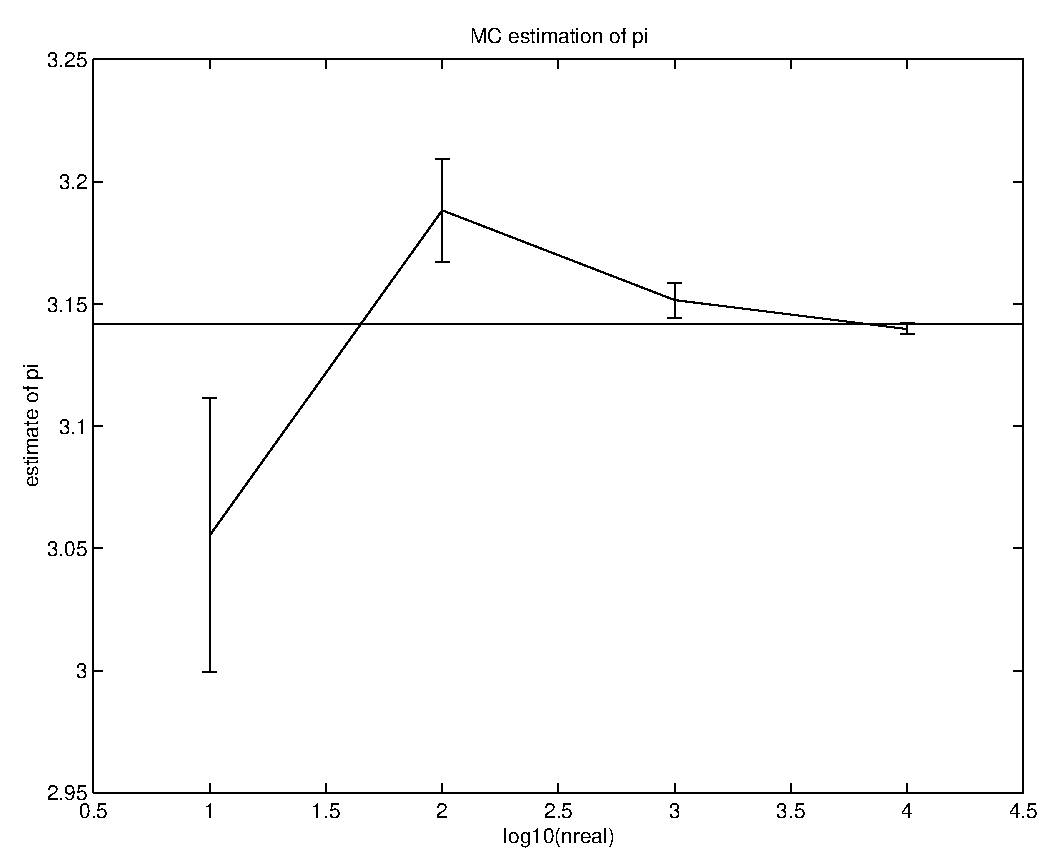
\includegraphics[width=\textwidth]{Figures/plotmcpi.eps}
\caption{The estimation of pi for n=10,100,1000,10000. The 
error bars correspond to the standard deviation of the mean of the 
estimate.}
\end{figure}

Next we write a program for the scoring  method. 

\subsubsection{Listing of the program mcpiscore.m}
\inputlisting{./Listings/mcpiscore.m}

Again we run the simulation for n=10, 100, 1000, 10000.
The result of a simulation can be seen in the next Figure.
\begin{figure}
\begin{center}
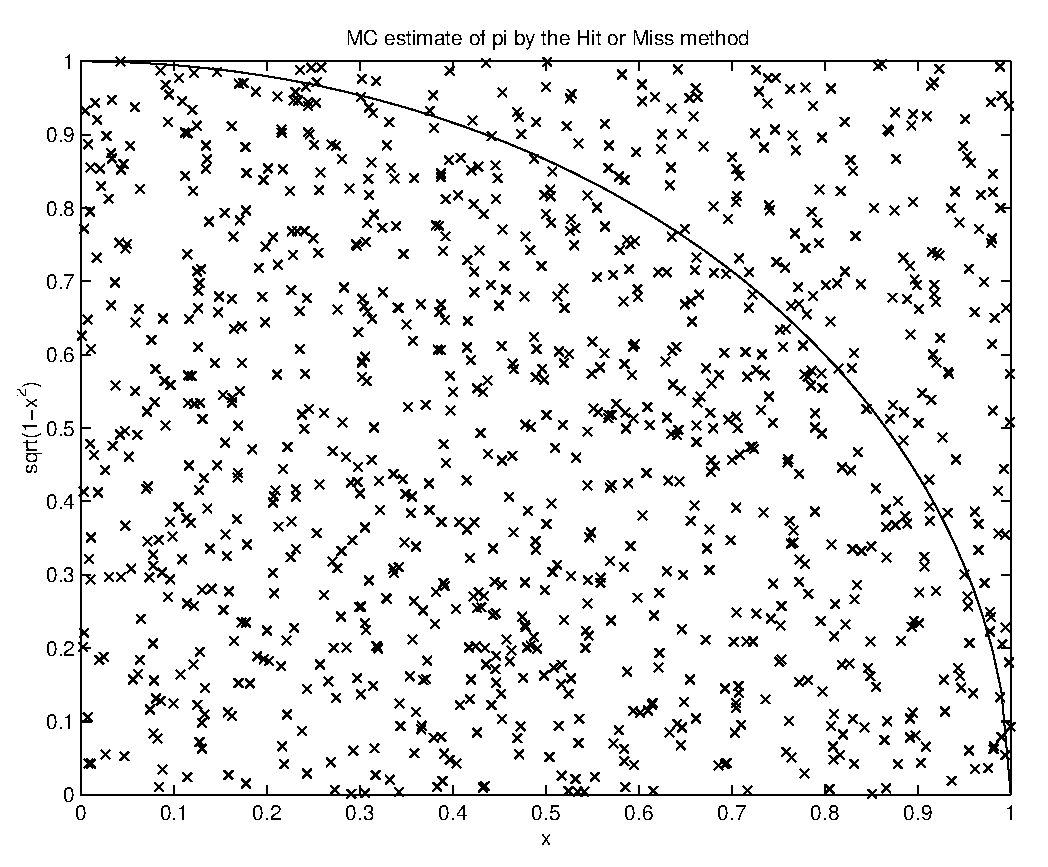
\includegraphics[width=.7\textwidth]{Figures/fmcpiscore.eps}
\end{center}
\caption{The scoring method. The continuous line represents
the function $\sqrt{(1-x^2)}$.}
\end{figure}


%%%%%%%%%%%%%%%%%%%%%%%%%%%%%%%%%%%%%%%%%%%%%%%%%%%%%%%%%%%%%%%%
\section{Beyond this chapter}


%%%%%%%%%%%%%%%%%%%%%%%%%%%%%%%%%%%%%%%%%%%%%%%%%%%%%%%%%%%%%%%%
\section{Exercises}

Use the  Matlab function \texttt{rand()}
to solve the following problems (don��t care about the quality and
the algorithm of the random number generator, for now):

\begin{Ex}
\label{Photoabsorption}
\textbf{Photoabsorption \cite[]{reif:67}} \\
Consider the absorption of photons passing through a gas in two dimensions.
We model the gas by introducing slabs of width $dx$ and density $n$ (in
particles per area), which absorb the incident photons. The slab
particles have a cross-sectional area of $\sigma$.

So the probability of a photon to be absorbed in the slab will be
($M$ is the number of particles in the slab of the height $dy$)
$$ P(\text{Photon absorbed}) = \frac{M\sigma}{dy} =
      \frac{\sigma n dx dy}{dy} = \sigma n dx  \quad .$$
We have assumed that there is no overlap between the cross-sections of
the slab particles.

Write a program to simulate this process on the computer. Take $N$
incident photons and watch the number of particles left over
against the slabs passed in a diagram. Do this simulation several
times and calculate the ensemble-average. What process you know
is similar to this behaviour and what takes the place of the spatial
dimension in that case?

%If we now have N identical slabs in a row, the probability of passing
%through all the slabs would be $(1-p)^N$, if the transmissions
%are statistically independent of each other.
%Then for a slab of finite thickness $X=N dx$ with $N\to\infty$, we
%get the Transmission probability
%$$ P(\text{transmitted through $N$ slabs}) =
%       \left(1-\frac{n\sigmaX}{N}\right)^N \quad .$$

%Now simulate the following systems:
%identical photons are absorbed in one slab ($N$ slabs)
\end{Ex}

\begin{Ex}
\label{Monte-Carlo_Integration}
\textbf{Monte-Carlo Integration -- Speed and Accuracy} \\
Write a program for the calculation of the following integral:
$$ \int_0^1 \frac{1}{1+x^2} dx\quad .$$
\begin{enumerate}
\item using the hit and miss method
\item using the standard method
\end{enumerate}
For both algorithms, calculate the mean and the standard deviation
as discussed in the lecture. Also use the analytical result of the
integral to calculate $\pi$. Compare the accuracy of both algorithms
using the approximations of $\pi$. Compare the speed of the two
programs by using the \texttt{cputime} function in Matlab.
(e.g. type the following to time the random number generator:
\texttt{t=cputime;x=rand(1000);cputime-t})

To that end, create a table and a plot with the two parameters
($n$: the number of intervals and $N$: the number of realizations)
against
the accuracy (use at least 5 values). To save time, you can first
check for a good $n$  and then do the plots only against $N$.
For the speed, plot the cputime against the achieved accuracy for
many different $N$.
\end{Ex}

\begin{Ex}
\label{Euler_Constant}
\textbf{Euler��s Constant using Monte-Carlo Algorithm %
          \cite[]{mohazzabi:98}} \\
Suppose throwing $N$ darts randomly at a dart board, which has been
divided into $R$ equal size regions. The probability of hitting one region
is $p=1/R$. Then the probability of hitting an empty region
(not already occupied by a dart) is $(1-p)^N$. Using the binomial
distribution, you can get the probability for hitting a region with
$m$ darts. If you choose
the number of regions equal to the number of darts
thrown on the board, we have $p=1/N$ and therefore
$$ P(\text{hitting an empty region}) = \left( 1-\frac{1}{N} \right)^N\quad .$$

Because the above series converges to $e$ for $N\to\infty$, we can use
the following method to get an approximation of the Euler constant:
\begin{enumerate}
\item[(i)] Throw randomly a large number of darts (say $N$) on a board, which has
  been divided into $N$ equal size regions.
\item[(ii)] Count the number of empty regions (call it $N_0$).
\item[(iii)] The fraction $N/N_0$ is a good estimate of the Euler constant $e$.
\end{enumerate}

Write a program for that algorithm and check the results. You can even
use $N/N_1$, if $N_1$ is the number of regions with the occupancy of
one dart. Check this, too. What $N$ do you need to
get the same accuracy using the formula? And how many terms of the
series for $e$ ($\sum_{i=0}^\infty 1/i! = e$)?
\end{Ex}

%%%%%%%%%%%%%%%%%%%%%%%%%%%%%%%


\bibliographystyle{peter}
\bibliography{V_98,simulit}

%%% Local Variables: 
%%% mode: latex
%%% TeX-master: "V_98"
%%% End: 
